\begin{figure}[h] 
\centering 
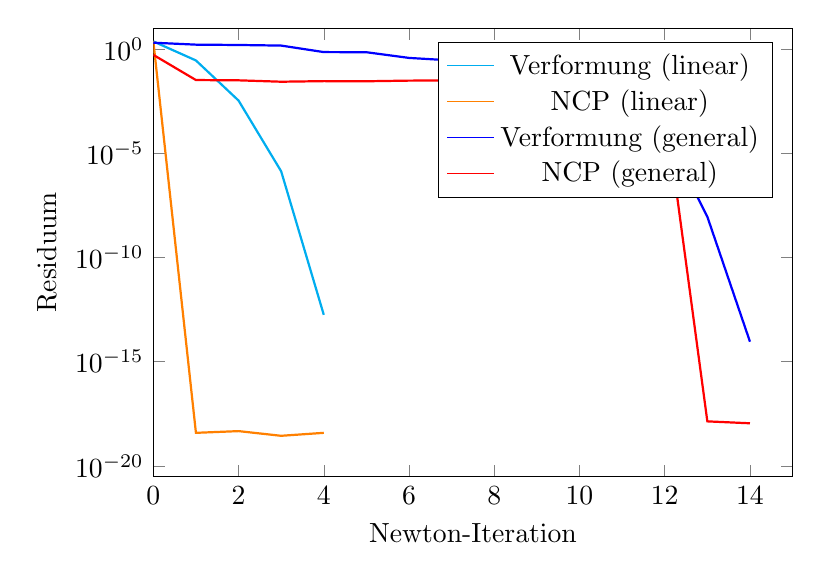
\begin{tikzpicture}[every plot/.append style={thick}] 
\begin{axis}[ 
label style={font=\normalsize}, 
xlabel={Newton-Iteration}, 
ylabel={Residuum}, 
xmin=0, xmax=15, 
ymode=log, 
ymin=0, ymax=10, 
width=0.8\textwidth, 
height=0.6\textwidth, 
legend pos=north east, 
legend style={cells={align=left}}, 
grid style=dashed, 
] 
\addplot[ 
color=cyan, 
] 
coordinates { 
(0, 2.33e+00)(1, 2.84e-01)(2, 3.38e-03)(3, 1.36e-06)(4, 1.77e-13)}; 
\addlegendentry{Verformung (linear)} 
\addplot[ 
color=orange, 
] 
coordinates { 
(0, 2.43e+00)(1, 3.83e-19)(2, 4.63e-19)(3, 2.76e-19)(4, 3.83e-19)}; 
\addlegendentry{NCP (linear)} 
\addplot[ 
color=blue, 
] 
coordinates { 
(0, 2.02e+00)(1, 1.63e+00)(2, 1.57e+00)(3, 1.47e+00)(4, 7.16e-01)(5, 7.05e-01)(6, 3.76e-01)(7, 2.85e-01)(8, 2.67e-01)(9, 2.83e-02)(10, 6.90e-03)(11, 8.75e-03)(12, 1.08e-04)(13, 8.99e-09)(14, 9.06e-15)}; 
\addlegendentry{Verformung (general)} 
\addplot[ 
color=red, 
] 
coordinates { 
(0, 5.28e-01)(1, 3.26e-02)(2, 3.16e-02)(3, 2.71e-02)(4, 2.89e-02)(5, 2.85e-02)(6, 3.06e-02)(7, 3.11e-02)(8, 1.02e-01)(9, 3.20e-02)(10, 3.21e-02)(11, 3.21e-02)(12, 2.28e-03)(13, 1.36e-18)(14, 1.10e-18)}; 
\addlegendentry{NCP (general)} 
\end{axis} 
\end{tikzpicture} 
\caption{Residuen des Stoffgesetzes 'Neo Hooke' mit Hinderniss 'Hut' und 578 Freiheitsgraden für die Verschiebung.} 
\label{fiq:NeoHooke_Hut_level3} 
\end{figure} 
